\documentclass[11pt]{standalone}
\usepackage{amssymb}
\usepackage{amsmath}
\usepackage[no-math]{fontspec}
\usepackage{unicode-math}
\usepackage{libertinus}
\usepackage{pgf,xcolor}
\usepackage{tikz}
\usetikzlibrary{arrows.meta, backgrounds}
\usepackage{pgfplots}
\pgfplotsset{compat=newest}

\definecolor{my_darkgray}{HTML}{484949}
\definecolor{my_lightgray}{HTML}{F3F4F4}
\definecolor{my_darkblue}{HTML}{005A94}
\definecolor{my_lightblue}{HTML}{CCDEE9}
\definecolor{my_yellow}{HTML}{FFEC7F}
\definecolor{my_red}{HTML}{E60000}
\definecolor{my_orange}{HTML}{E87846}

\begin{document}
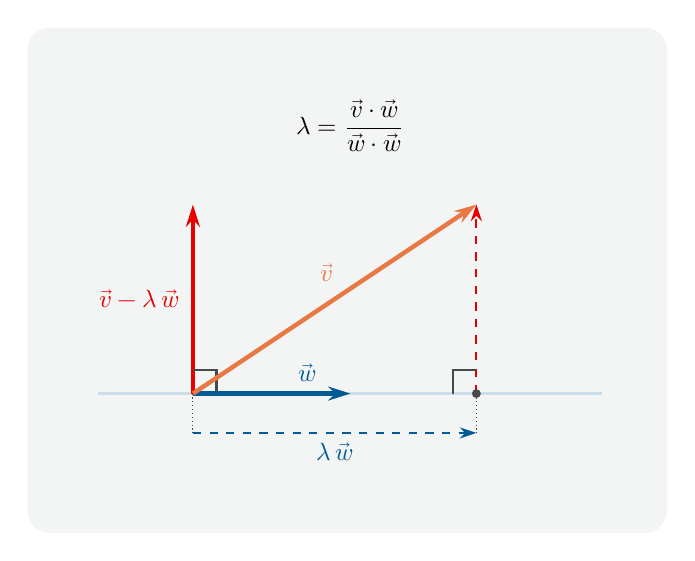
\begin{tikzpicture}[
    show background rectangle,
    background rectangle/.style={fill=my_lightgray, rounded corners=8pt},
    inner frame sep=0.8cm,
    x=1cm, y=1cm,
    vec/.style={-{Stealth[length=8pt, width=5pt]}, ultra thick},
    weg/.style={-{Stealth[length=6pt, width=4pt]}, thick, dashed}
]

% ---------------------------------------------------------------
%  Projektion von v = (3.6, 2.4) auf w = (2, 0)
%    lambda = (v.w)/(w.w) = 7.2/4 = 1.8,   lambda w = (3.6, 0)
%    Rest v - lambda w = (0, 2.4)
% ---------------------------------------------------------------

% Gerade durch w
\draw[my_lightblue, very thick] (-1.2, 0) -- (5.2, 0);

% Projektion lambda w, leicht unterhalb der Geraden
\draw[my_darkgray, densely dotted] (0, 0) -- (0, -0.5);
\draw[my_darkgray, densely dotted] (3.6, 0) -- (3.6, -0.5);
\draw[weg, my_darkblue] (0, -0.5) -- (3.6, -0.5);
\node[below, font=\small, my_darkblue] at (1.8, -0.5) {$\lambda\,\vec{w}$};

% Rest v - lambda w im Ursprung und verschoben an den Lotfusspunkt
\draw[vec, my_red] (0, 0) -- (0, 2.4);
\node[left, font=\small, my_red] at (-0.05, 1.2) {$\vec{v} - \lambda\,\vec{w}$};
\draw[weg, my_red] (3.6, 0) -- (3.6, 2.4);

% rechte Winkel im Ursprung und im Lotfusspunkt
\draw[my_darkgray, thick] (0.3, 0) -- (0.3, 0.3) -- (0, 0.3);
\draw[my_darkgray, thick] (3.3, 0) -- (3.3, 0.3) -- (3.6, 0.3);
\fill[my_darkgray] (3.6, 0) circle (1.6pt);

% Vektor w
\draw[vec, my_darkblue] (0, 0) -- (2, 0);
\node[above, font=\small, my_darkblue] at (1.45, 0.02) {$\vec{w}$};

% Vektor v
\draw[vec, my_orange] (0, 0) -- (3.6, 2.4);
\node[above left, font=\small, my_orange] at (1.9, 1.3) {$\vec{v}$};

\node[font=\small] at (2, 3.4)
    {$\lambda = \dfrac{\vec{v}\cdot\vec{w}}{\vec{w}\cdot\vec{w}}$};

\end{tikzpicture}
\end{document}
